\subsubsection{Job System}

For asynchronous compilation to be possible, the hybrid emulator requires multiple threads in some capacity. Spawning a new thread for every compilation would be a particularly bad idea for several reasons, including but not limited to:

\begin{itemize}
    \item The overhead for creating and destroying threads is particularly high
    \item Creating more threads than the system has logical processors will lead to unnecessary contention and performance degradation
\end{itemize}

For these reasons, a thread pool was developed, as outlined in \autoref{figure:job-system}. This provides a highly flexible and efficient API for deferring work, packaged as jobs, to worker threads. The caller (in this case the hybrid emulator) gives the thread pool jobs which are then stored in a concurrent job queue; the worker threads will then fetch jobs from these queue, process them, then emit the results of the job to a second concurrent results queue. The main thread can then consume results from the queue at a time that is appropriate for it.

\begin{figure}[h]
    \centering
    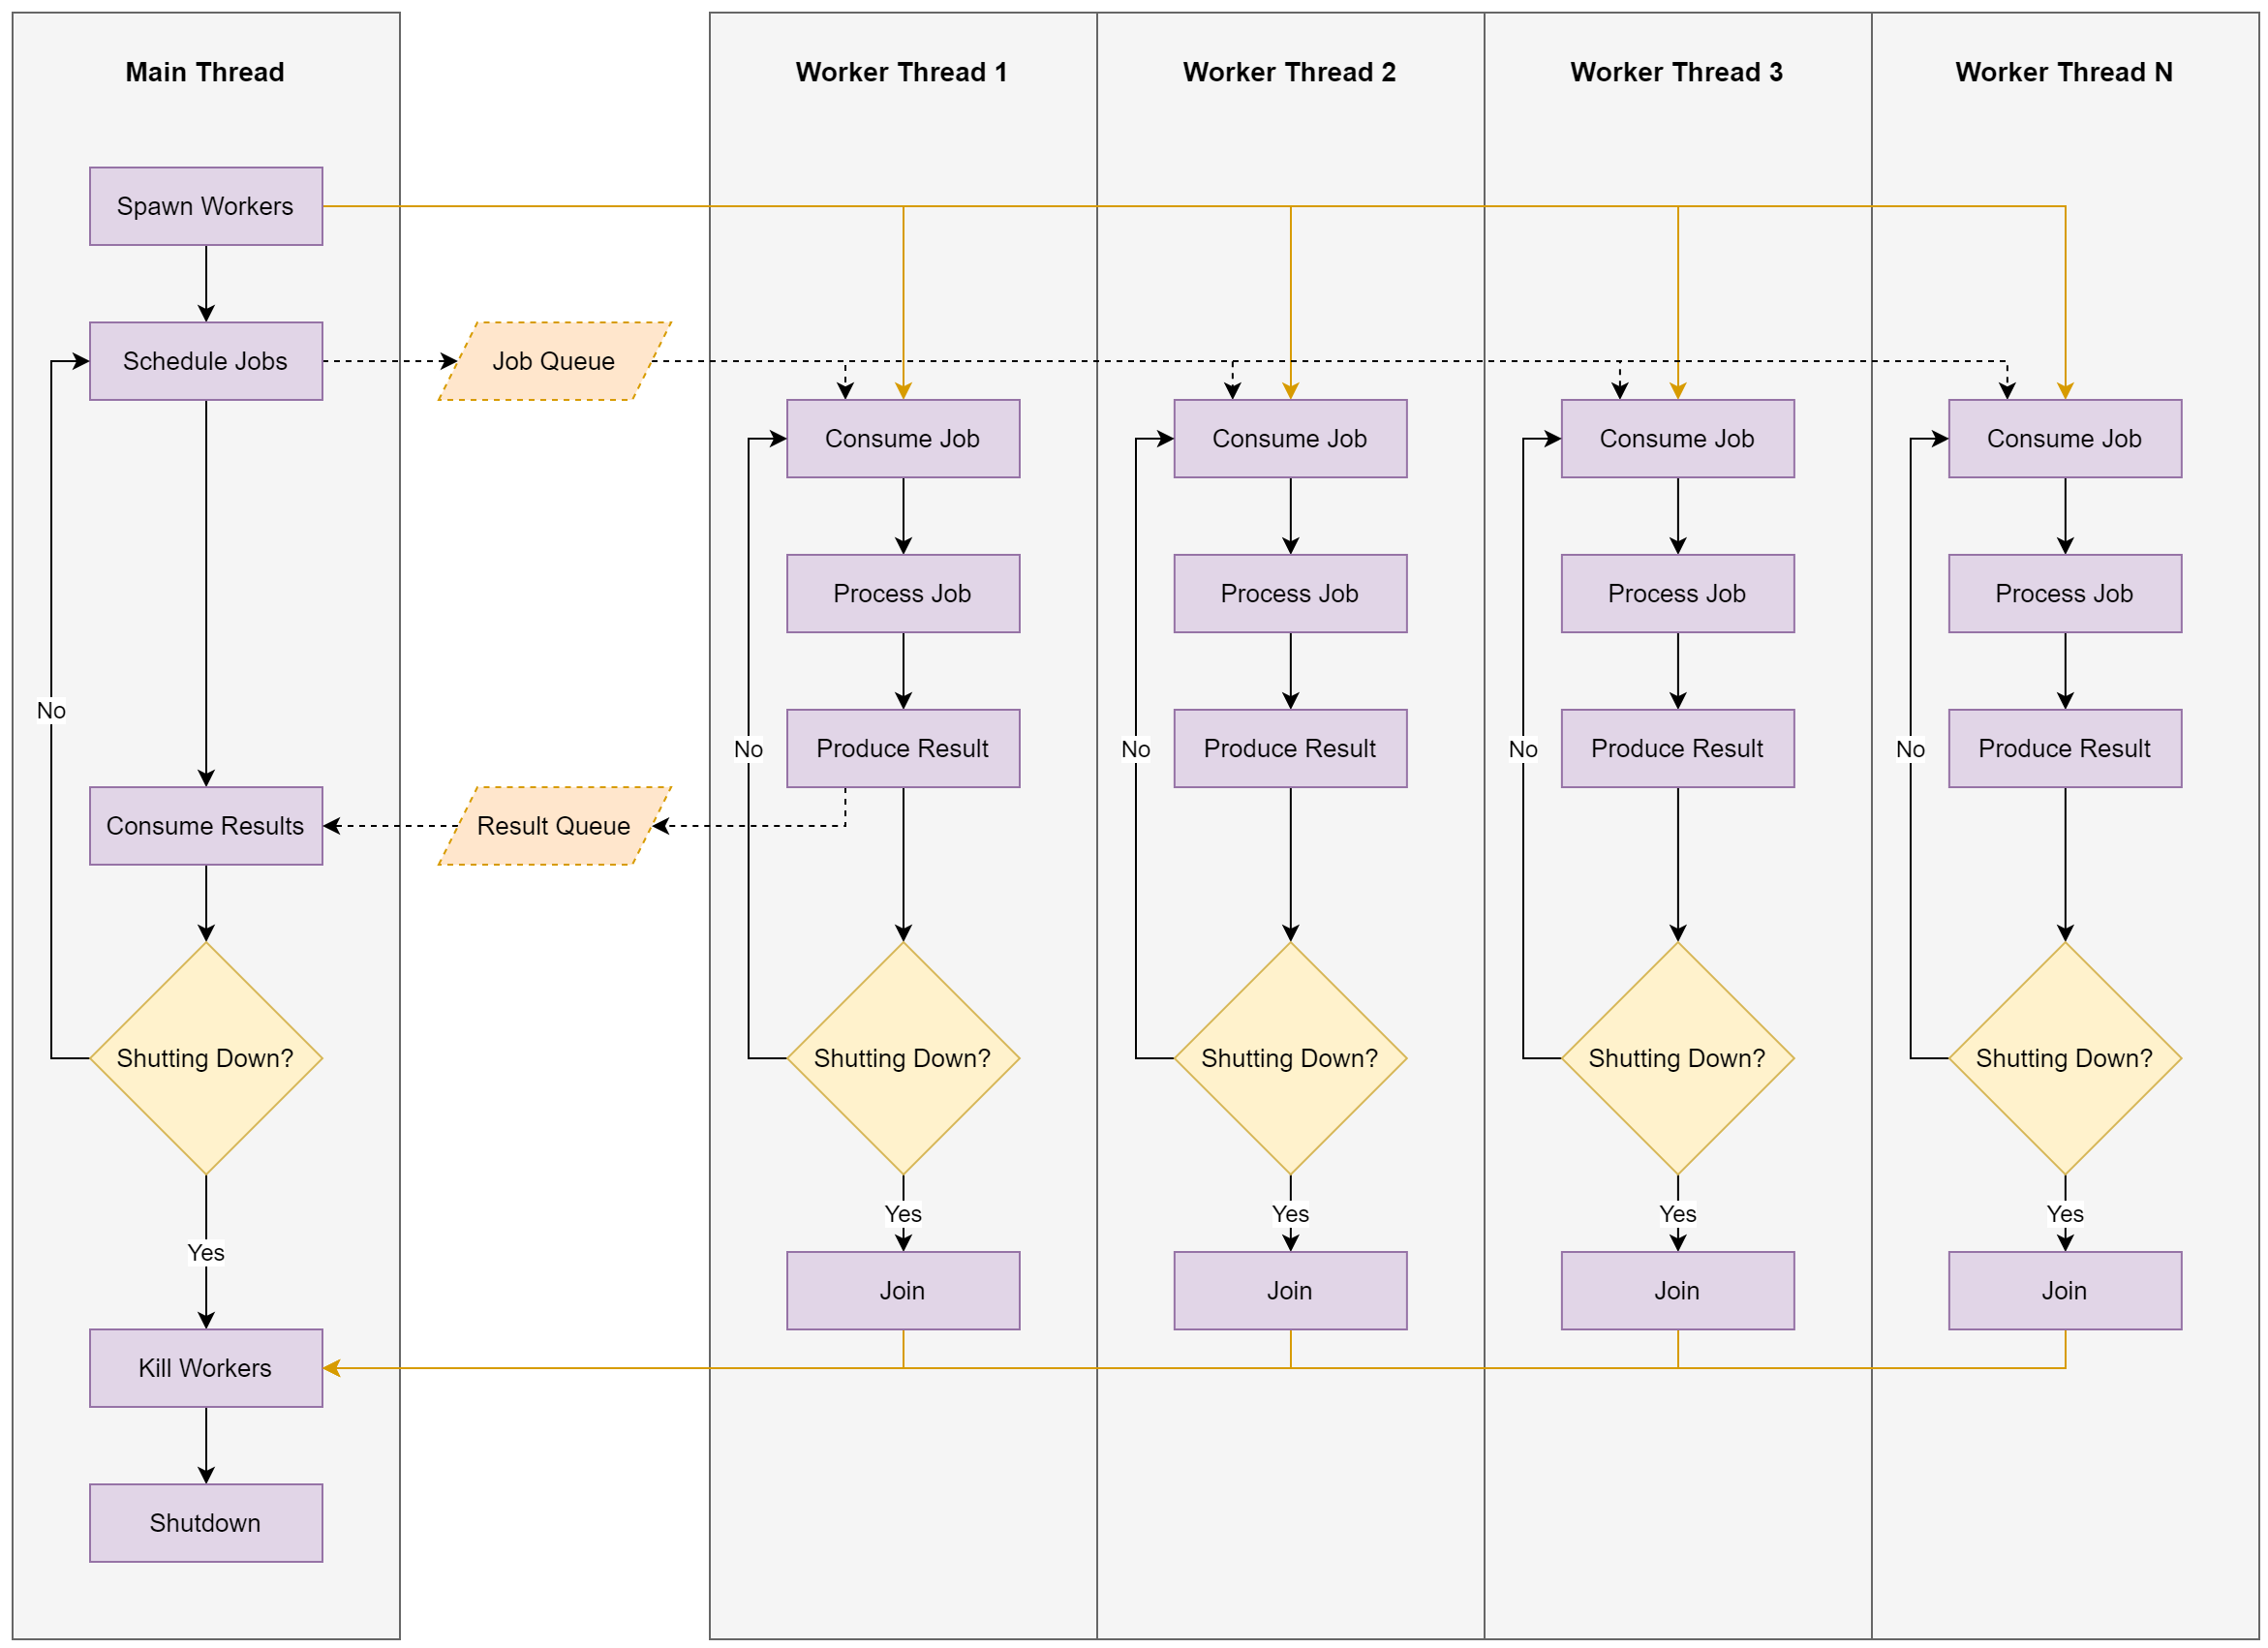
\includegraphics[width=1\linewidth]{diagrams/thread-pool.png}
    \caption{The job system developed for offloading work from the main thread to many worker threads.}
    \label{figure:job-system}
\end{figure}

This job system approach has a variety of benefits. It helps decouple the asynchronous job from the main thread that requires the work; minimising the overlap of state between threads is key in concurrent programming to help avoid the array of concurrency bugs that are typical of the field. By using the results queue, instead of having the worker threads themselves act on the results, we can delegate the stateful changes to the main thread, localising the state to a single thread.

\autoref{code:schedule-job} shows the typical caller code for scheduling a job on a thread pool. The job queue is automatically managed by the thread pool whereas the results queue is managed by the caller, as shown in \autoref{code:consume-results}.

\begin{lstfloat}[H]
    \begin{lstlisting}[language=c++]
auto& thread_pool = common::Enviornment::get().thread_pool();
thread_pool.schedule_job(threading::Job([&]
{
    // do work
    _result_queue.enqueue(/* results */);
}));
    \end{lstlisting}
    \caption{Typical caller code for scheduling a job on the thread pool.}
    \label{code:schedule-job}
\end{lstfloat}

\begin{lstfloat}[H]
    \begin{lstlisting}[language=c++]
Result result;
while (_result_queue.try_dequeue(result))
{
    // process result
}
    \end{lstlisting}
    \caption{Typical caller code for consuming results produced by thread pool.}
    \label{code:consume-results}
\end{lstfloat}

The thread pool will lazily initialize more worker threads if the number of pending jobs exceeds the number of free workers, up to a maximum of \texttt{N-1} workers, where \texttt{N} is the number of logical processors on the system. The lazy initialization helps avoid the overhead of thread creation in workloads that do not require extra workers, and the maximum worker count avoids excessive thread contention.

The thread pool should be created once and used globally for the entire processes' lifetime. This avoids contention between multiple thread pools and minimises the cost associated with creating and killing threads. This was achieved by having a global \texttt{Enviornment} which was encapsulated through a lazy-initialised singleton pattern; this \texttt{Enviornment} then contains the thread pool and any other global instances required.

\YIComment{maybe explain singleton}

\YIComment{moodycamel} \cite{moodycamel, moodycamel-benchmark}

\YIComment{Talk about results queue optimisation}